\documentclass[a4paper,11pt,lualatex,ja=standard]{bxjsarticle}

% 数式
\usepackage{amsmath,amsfonts}
\usepackage{bm}
% 画像
\usepackage{graphicx}
% url
\usepackage{hyperref}

% ===== cover command =====
\newcommand{\cover}[3]{
  \thispagestyle{empty}
  \vspace*{4cm}
  \begin{center}
    {\LARGE #1}\\[2cm]
    {\Large #2}\\[3cm]
    {\large 氏名：#3}\\[1cm]
    {\large 学籍番号：s2510063}
  \end{center}
  \newpage
}
% =========================

\begin{document}

% ===== cover =====
\cover{Perceptron Train XOR}{SyLab}{小林智輝}
% =================

\title{レポートタイトル}
\author{氏名}
\date{\today}

\section{問題文}
\begin{verbatim}
Watch a perceptron learn in real time on XOR data using the classic update rule: only misclassified points trigger updates, 
with no weight decay. Because XOR is not linearly separable, 
a single perceptron cannot hit 100% accuracy. 
Reach 75% accuracy to prove you understand the limitation and reveal the flag.
\end{verbatim}


\begin{figure}[h]
  \centering
  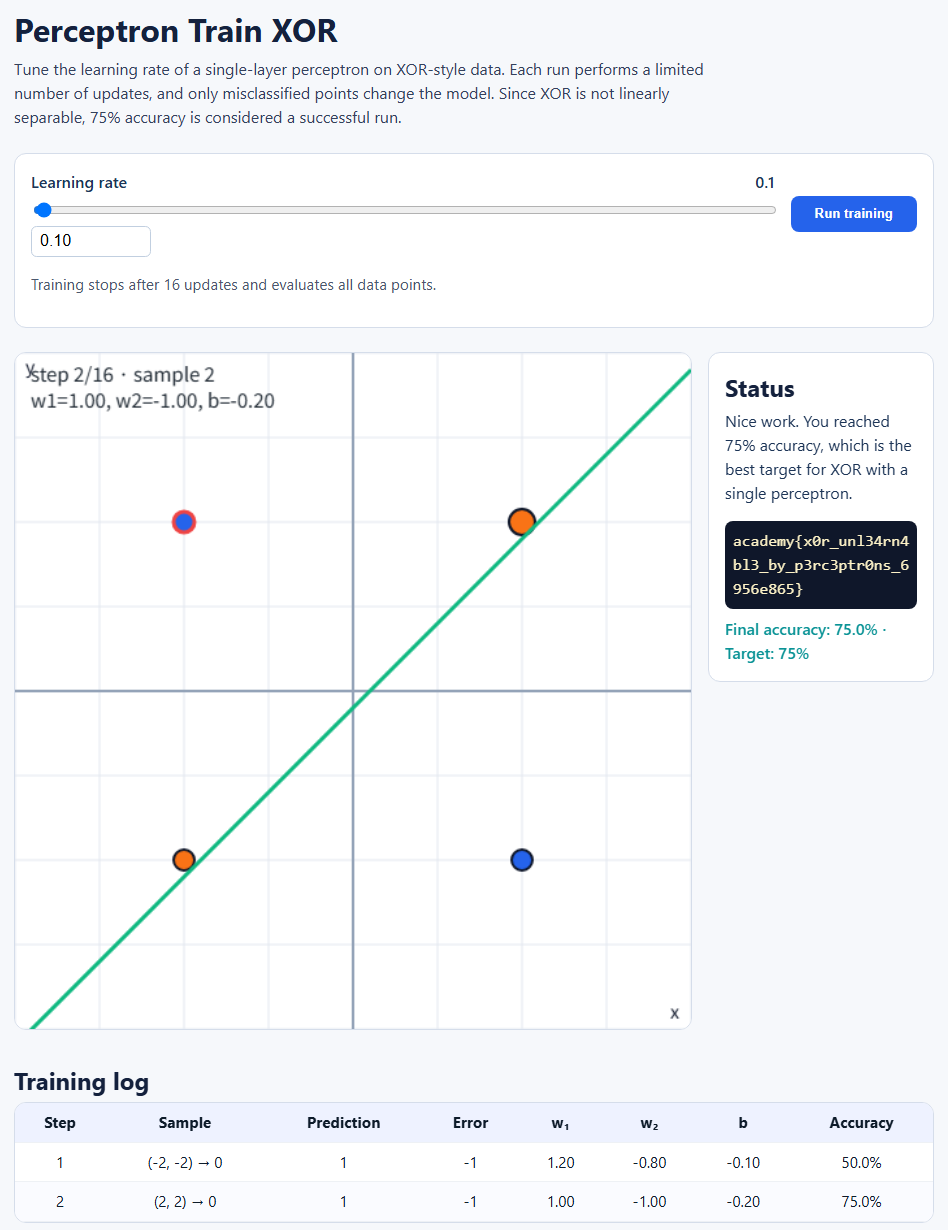
\includegraphics[width=0.7\linewidth]{01.png}
  \caption{img}
\end{figure}

\end{document}